\section{Flächen in Kartesische Koordinaten}

\begin{itemize}
    \item\textit{Eine Fläche S ist eine \textbf{Regelfläche} falls durch jeden ihrer Punkte eine Gerade existiert, die vollständig in S liegt.}
    \item\textit{\textbf{doppelte Regelfläche} falls durch jeden ihrer Punkte zwei unterschiedliche Geraden existieren}
\end{itemize}



\textbf{Explizite Darstellung} \\
\textit{Sattel:}
$z = f(x,y) = x^2 - y^2$ \\
\\
\textbf{Implizite Darstellung} \\
\textit{Kugel:}
$(x-x_0)^2 + (y-y_0)^2 + (z-z_0)^2 = R^2$ \\
\textit{$x_0$, $y_0$, $z_0$ = Zentrum}
\\
\textbf{Parameterdarstellung} \\

Zylinderkoordinaten:
\textit{$(r,\theta,z)$}
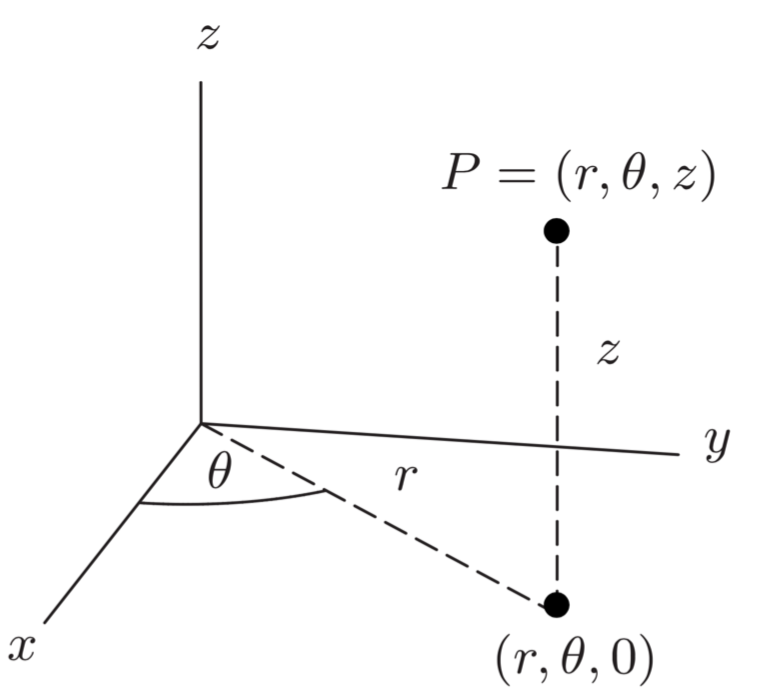
\includegraphics[width=0.3\textwidth]{assets/Zylinderkoordinaten.png}
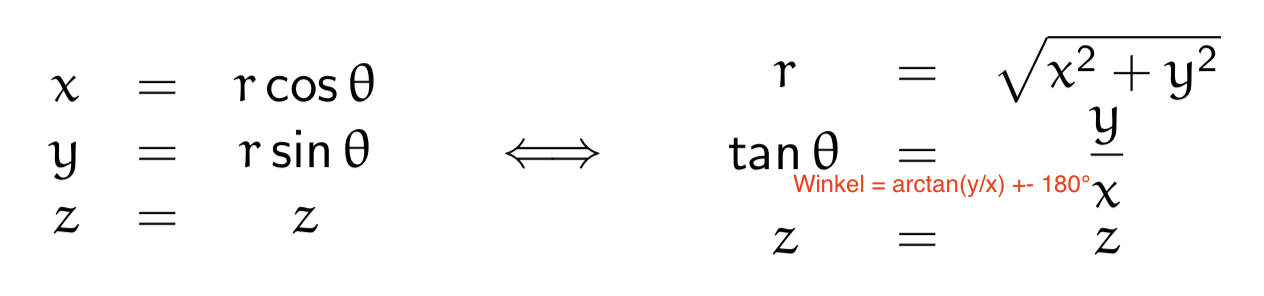
\includegraphics[width=0.4\textwidth]{assets/ZylinderkoordinatenUmrechnnung.png}

Kugelkoordinaten:
\textit{$(\rho,\phi,\theta)$}
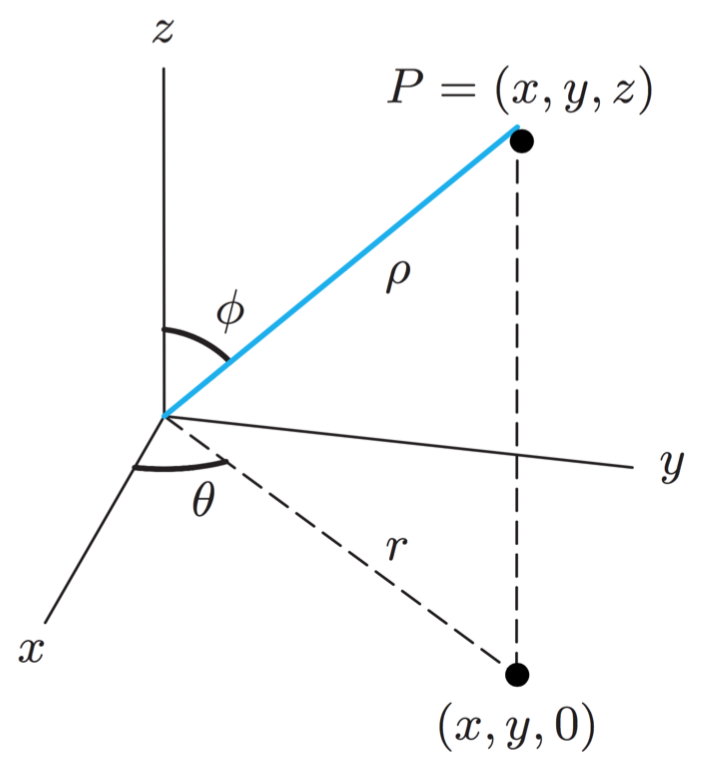
\includegraphics[width=0.3\textwidth]{assets/Kugelkoordinaten.png}
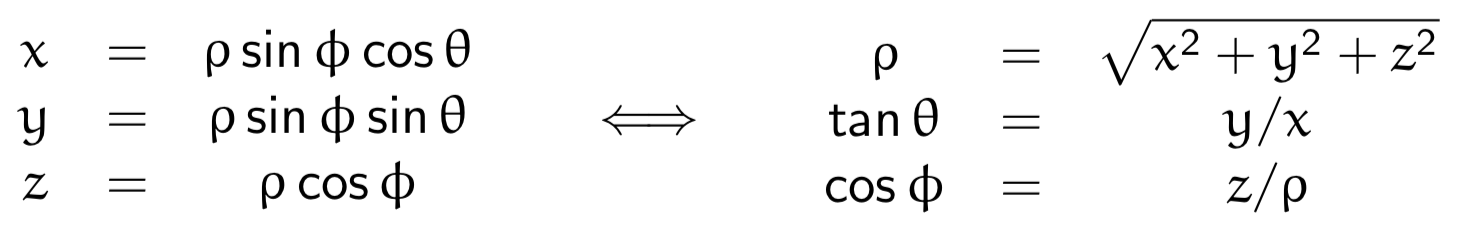
\includegraphics[width=0.4\textwidth]{assets/KugelkoordinatenUmrechnung.png}

Rotationsfläche:\\
\textit{$x=u$}\\
\textit{$y = f(x) * cos(v)$}\\
\textit{$z = f(x) * sin(v)$}\\

\textit{Beispiel Beschreibung Fläche mit Zylinderkoordinaten:}\\
$T_B = \{(r, \theta, 0)|0 \leq r \leq 6 \wedge 0 \leq \theta \leq \frac{\pi}{6}\}$\\

\textit{Beispiel Beschreibung Fläche mit Kugelkoordinaten:}\\
$M = \{(\rho, \frac{\pi}{4}, \theta)|0 \leq \rho \leq 1 \wedge 0 \leq \theta \leq 2\pi\}$

\textit{Parametrisieren eines Kegels von den Aufgaben:}
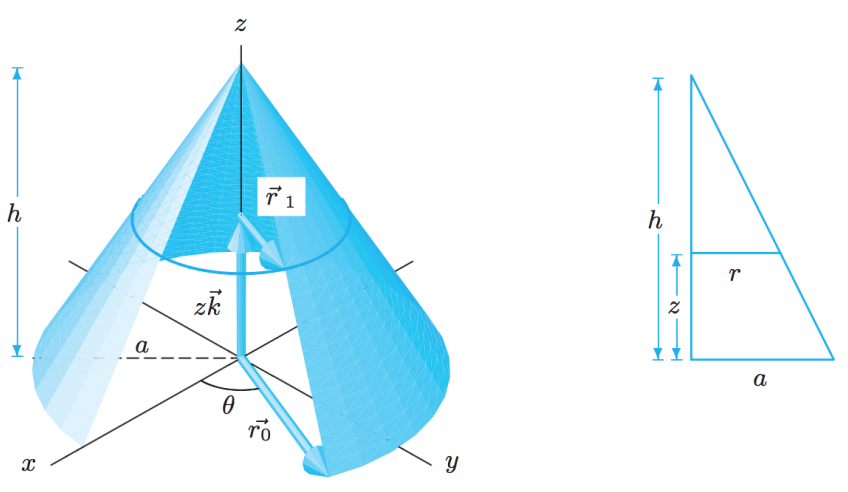
\includegraphics[width=0.45\textwidth]{assets/area-parameterize-example.png}

\textit{Mit definition Einheitsvektoren x ($\vec{i}$), y ($\vec{j}$) und z ($\vec{k}$) Richtung}\\
$\vec{r}(\theta, z) = \vec{r}_1 + z\vec{k} =
a(1-\frac{z}{h}) (\cos(\theta)\vec{i} + \sin(\theta)\vec{j}) + z \vec{k}$\\

\textit{Alternativ schreibweise:} \\
$x(\theta,z) a(1-\frac{z}{h}) \cos (\theta)$ \\
$y(\theta,z) a(1-\frac{z}{h}) \sin (\theta)$ \\
$z=z$

\subsection{Freiformflächen}

\textit{Handelt sich dabei und den selben Ansatz wie bei den Kurven,
nur auf flächen, siehe Kurven:}\\

$F(u) = \displaystyle \sum^n_{i=0}(C_i N_i (u))$, $0 \leq u \leq 1$\\
\textit{Kurve $F(u)$ mit Grad $n$}\\
$G(u) = \displaystyle \sum^m_{j=0}(C_j N_j (v))$, $0 \leq v \leq 1$\\
\textit{Kurve $G(u)$ mit Grad $m$}\\

$S(u,v) = \displaystyle \sum^n_{i=0}\sum^m_{j=0}(C_iC_jN_i(u)N_j(v))$, $0 \leq u, v \leq 1$\\
\textit{$S(u,v)$ definiert die Tensorproduktfläche}

\textit{Wobei $C_i$, $C_j$ Kontrollpunkte sind und $N_i$, $N_j$ die Splineformel}

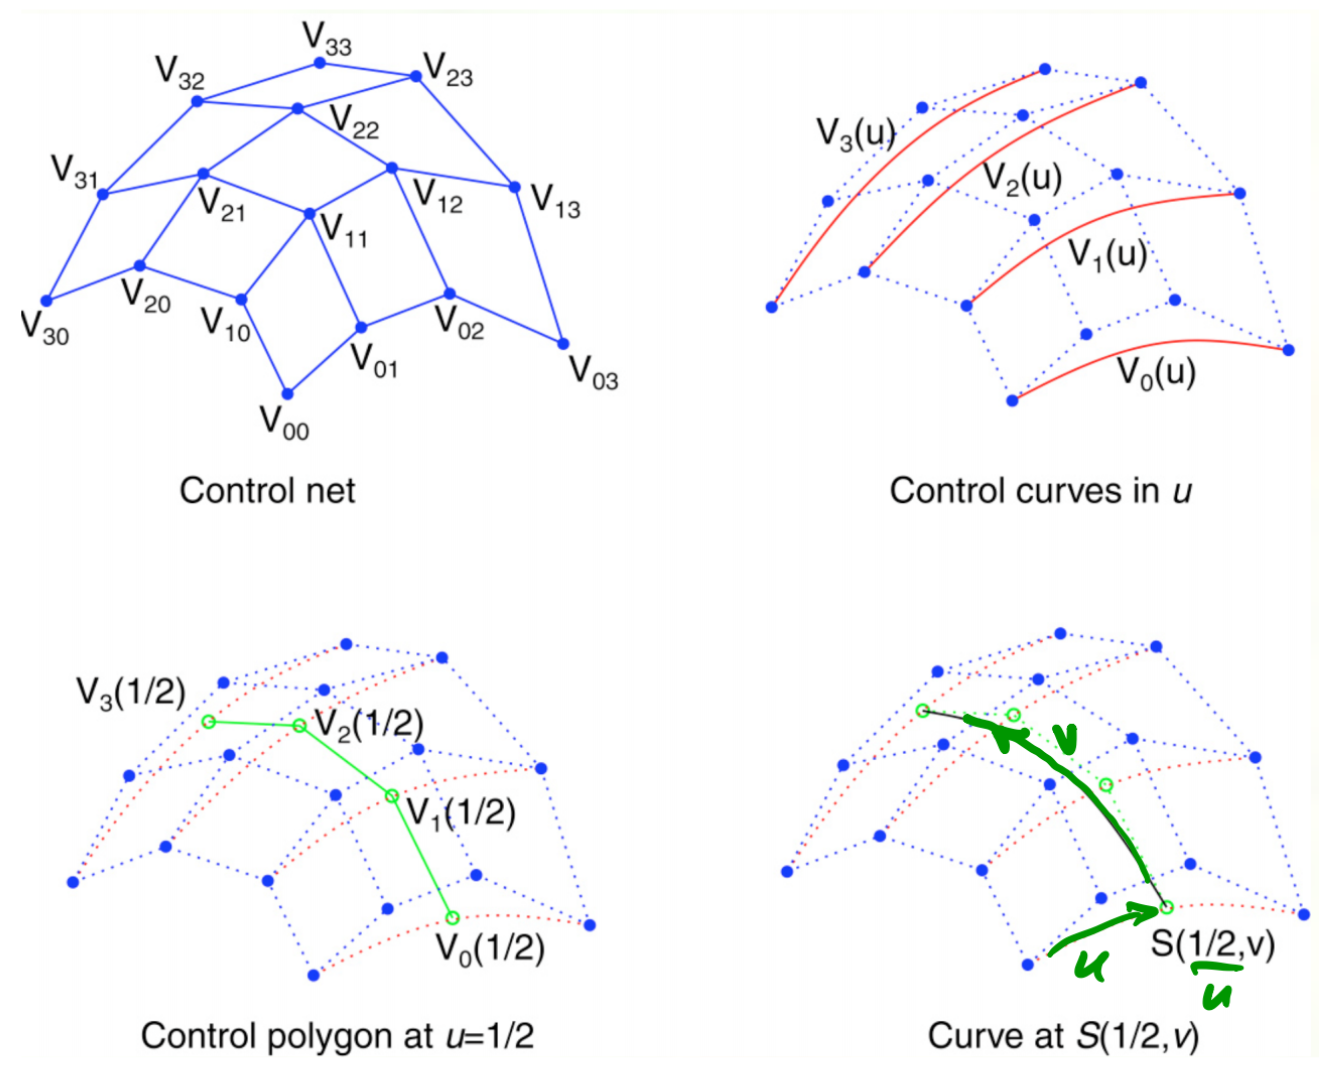
\includegraphics[width=0.5\textwidth]{assets/area-splines.png}

\textit{Die Freifläche lässt sich auch gleich durch die Bézier-Kurven definieren:}\\

$Q(u,v)= \displaystyle \sum^n_{i=0}\sum^m_{j=0}B^n_i(v) \cdot B_j^m(u) \cdot P_{i,j}$\\
$B_i^n(v) = \left(\begin{matrix}
    n \\ i
\end{matrix}\right) (1 - v)^{n-i}v^i$, $(0 \leq i \leq n)$\\
$B_j^m(u) = \left(\begin{matrix}
    m \\ j
\end{matrix}\right) (1 - u)^{m-j}u^j$, $(0 \leq j \leq m)$

\subsection{Matrixdarstellung Bézier-Fläche}

$U=[1,u,u^2,u^3]$\\
$V=[1,v,v^2,v^3]$\\
$M=\begin{bmatrix}
    1 & 0 & 0 & 0 \\
   -3 & 3 & 0 & 0 \\
    3 &-6 & 3 & 0 \\
   -1 & 3 &-3 & 0 \\
\end{bmatrix}$\\
$G = \begin{bmatrix}
    P_{0,0} & P_{0,1} & P_{0,2} & P_{0,3} \\
    P_{1,0} & P_{1,1} & P_{1,2} & P_{1,3} \\
    P_{2,0} & P_{2,1} & P_{2,2} & P_{2,3} \\
    P_{3,0} & P_{3,1} & P_{3,2} & P_{3,3} \\
\end{bmatrix}$\\

$P(u,v) = UMGM^TV^T$\\
$P_i(u,v) = UMG_iM^TV^T$, $(i = x,y,z)$

\begin{itemize}
    \item Tensorproduktfläche S(u,v) = Fläche gegeben von Kurven F(u) \& G(v) \\
    \textit{Für jeden u Wert gibt es eine Kurve -> "Gitterpunkte"}
\end{itemize}